\chapter{A Teoria da Medida}
%%%%%%%%% ESPAÇOS MENSURÁVEIS
    Nesta seção, apresentaremos o conceito chave deste trabalho: a teoria da medida.
    %Conhecemos este conceito de forma intuitiva pelo o que vemos, geralmente, na geometria euclidiana plana.
    %Aqui, trataremos de medida de modo generalizado. 
    Para isso, precisaremos ampliar o conjunto dos números reais para que ele possa atender novas exigências.
    Isso é necessário porque, as vezes, teremos conjuntos tão \enquote{grandes} que nenhum número real poderá representar sua \enquote{medida}. 
    Assim, estenderemos o conjunto dos números reais na primeira seção.
    Na seguinte, estenderemos o conceito de função mensurável para o conjunto dos números reais estendidos e, na seção final, apresentaremos a definição de medida bem como exemplos dela.
    
\section{Os Espaços de Funções Mensuráveis}
	Adiante apresentaremos conjuntos tão \enquote{grandes} que nenhum número real poderá expressar seu \enquote{tamanho}.
	Assim, antes de prosseguirmos expandiremos o conjunto da reta real que temos trabalhado anteriormente.
    \begin{env}{Definição}
    \label{def:reta-estendida}
        O conjunto $\xreta$ que consiste de $\R \cup \{-\infty, +\infty\}$ é chamada de \textbf{Sistema Estendido de Números Reais}
        \cite[p.5, tradução nossa]{bartle}
        \footnote{No original: The collection $\xreta$ consisting of
        	the set $\R \cup \{ -\infty , + \infty\}$ is called the extended real number system.}.
    \end{env}

    Ou seja, $\xreta$ nada mais é que o conjunto dos números reais com a possibilidade de se ter $-\infty$ ou $+\infty$.
    Com isso, parece que nosso problema de \enquote{medir} conjuntos muito grandes se resolveu.
    Entretanto, alguns cuidados são necessários para operarmos em $\xreta$.
    Um deles, por exemplo, é que $\xreta$ não é fechado para operações de $\R$ tais como $(+\infty) + (-\infty)$.
    Dito isso, para $x \in \R$, as operações dos símbolos $+\infty$ e $-\infty$ são dadas da seguinte forma:
    \vspace{-0.4cm}
    \begin{multicols}{2}
        \begin{itemize}
            \item $(+ \infty) + (+ \infty)  = + \infty$;
            \item $x + (+ \infty) = (+ \infty) + x = + \infty$;
            \item $(- \infty) + (- \infty)  = - \infty$;
            \item $x + (- \infty) = (- \infty) + x = - \infty$;
            \item $(+ \infty)\cdot (+ \infty) =  +\infty $;
            \item $(- \infty)\cdot (- \infty) =  +\infty $;
            \item $(+ \infty)\cdot (- \infty) =  -\infty $;
            \item $(- \infty)\cdot (+ \infty) =  -\infty $.
        \end{itemize}
    \end{multicols}
	
	\vspace{-0.4cm}
    Na multiplicação, dependendo do número real, a operação diferencia-se.
    Assim, podemos ter
    \vspace{-1cm}
    \begin{multicols}{2}
    $$
    x \cdot (+\infty) = (+\infty) \cdot x =
    \left\{\begin{array}{cc}
          +\infty, & \ \textrm{se } x > 0\\
          0, & \ \textrm{se } x = 0\\
          - \infty, & \textrm{se } x < 0
    \end{array}\right.
    $$
    
    $$
    x \cdot (-\infty) = (-\infty) \cdot x =
    \left\{\begin{array}{cc}
          -\infty, & \ \textrm{se } x > 0\\
          0, & \ \textrm{se } x = 0\\
          + \infty, & \textrm{se } x < 0
    \end{array}\right.
    $$  
    \end{multicols}
	\vspace{-0.4cm}
    Neste novo contexto de números reais a \sigal de Borel não é mais válida uma vez que a \ref{def:algebra-borel} não inclui $+\infty$ nem $-\infty$.
    Logo, precisaremos de uma $\sigma$-álgebra em $\xreta$ para dar continuidade aos nossos estudos. 
    Com isso, considere $\xreta$.
    Tomando um conjunto arbitrário $E \in \borel$, com $\varnothing \neq E$, defina $E_1 = E \cup \{-\infty\}, E_2 = E \cup \{+\infty\}$ e $E_3 = E \cup \{-\infty, +\infty\}$. Com isso podemos fazer o seguinte enunciado: 
    % Desta forma, o conjunto $\overline{\borel} = \displaystyle \bigcup_{E \in \borel} \{E, E_1, E_2, E_3\}$ é uma \sigal de $\xreta$.
    \begin{comment}
    Com efeito, se $E \in \borel$, então é um intervalo aberto conforme o teorema \ref{teo:equiv-borel}.
    Assim, $E_1, E_2, E_3$ e $E_4$ serão intervalos do tipo $[-\infty,x)$ ou $(x, +\infty]$ que são elementos de $\borel$ acrescidos de $+\infty$ ou $-\infty$. 
    Deste modo, é fácil verificar que se um elemento $A \in \xborel$, então $A^c \in \xborel$.
    Além disso, a união enumerável é, no máximo, o intervalo $[-\infty,+\infty]$ que é exatamente $\xreta$.
    Desta forma, $\xborel$ é uma \sigal de $\xreta$.
    	
    \end{comment}
    
    \begin{env}{Definição}
    \label{def:algebra-borel-estendida}
        A \sigal $\overline{\borel} = \displaystyle \bigcup_{E \in \borel} \{E, E_1, E_2, E_3\}$ do conjunto $\xreta$ é chamada de Álgebra de Borel Estendida \cite{bartle}.
    \end{env}

    Uma vez que estamos familiarizados com os conceitos de funções de valores reais mensuráveis, estamos prontos para estender este conceito para o conjunto $\xreta$.
    \begin{env}{Definição}
    \label{def:familia-funcoes-mensuraveis}
        Sendo $(X, \mathcal{C})$ um espaço mensurável, uma função de valores reais estendidos $f: X \to \xreta$ é dita $\mathcal{C}$-mensurável caso o conjunto
        $\{x \in X; f(x) > \alpha\} \in \mathcal{C}$ para qualquer que seja $\alpha \in \R$ \cite{bartle}. 
        \vspace{-0.4cm}
    \end{env}

	Denotaremos a família de todas as funções de valores reais estendidos de $X$ que são $\mathcal{C}$-mensuráveis por $M(X, \mathcal{C})$.
	Além disso, caso estivermos tratando apenas das funções não negativas usaremos $M^+(X, \mathcal{C})$.
    \begin{env}{Proposição}
    \label{prop:identidade-intersecao-mais-infinito}
        Se $f \in \menfus$, então $\{x \in X; f(x) = +\infty\} = \displaystyle \bigcap_{n = 1}^\infty \{x \in X; f(x) > n\}$
        \cite{bartle}.
    \end{env}
    \begin{prova}
        Tome, de modo arbitrário, um elemento $a \in X$. 
        Assim, 
        \begin{align*}
            a \in \bigcap_{n = 1}^\infty \{x \in X; f(x) > n\} 
            \Leftrightarrow &\ a \in \{x \in X; f(x) > n\}, \ \forall\  n \in \N\\
            \Leftrightarrow &\  \forall\ n \in \N,\ f(a) > n\\
            \Leftrightarrow & f(a) = +\infty.  
        \end{align*}
    Além disso, note que cada $\{x \in X;\, f(x) > n\} \in \mathcal{C}$.
    Segue, pela \ref{prop:interseção-elementos-sigmas}, que \linebreak $\displaystyle \bigcap_{n = 1}^\infty \{x \in X; f(x) > n\} \in \mathcal{C}$ acarretando que $\{x \in X; f(x) = +\infty\} \in \mathcal{C}$. 
    \end{prova}

    \begin{env}{Proposição}
    \label{prop:identidade-união-menos-infinito}
        Se $f \in \menfus$, então $\{x \in X; f(x) = -\infty\} = \displaystyle \left(\bigcup_{n = 1}^\infty \{x \in X; f(x) > - n\}\right)^c$
        \cite{bartle}.
        \vspace{-0.4cm}
    \end{env}
	%
    \begin{prova}
    	
    	\vspace{-0.6cm}
        Analogamente à \ref{prop:identidade-intersecao-mais-infinito} tomemos $a \in X$. 
        Segue que 
        \begin{align*}
            a \in \left(\bigcup_{n = 1}^\infty \{x \in X; f(x) > - n\}\right)^c
            \Leftrightarrow & \ a \in \bigcap_{n = 1}^\infty \left(\{x \in X; f(x) > - n\}\right)^c\\
            \Leftrightarrow & \ \forall \ n \in \N,\ a \in \left(\{x \in X; f(x) > - n\}\right)^c\\
            \Leftrightarrow & \ \forall \ n \in \N,\ a \notin \{x \in X; f(x) > - n\}\\
            \Leftrightarrow & \ \forall \ n \in \N,\ a \in \{x \in X; f(x) \leq - n\}\\    
            \Leftrightarrow & \ \forall \ n \in \N,\ f(a) \leq - n\\
            \Leftrightarrow & \lim_{n \to \infty} f(a) \leq \lim_{n \to \infty} (- n)\\  
            \Leftrightarrow & f(a) = -\infty.                  
        \end{align*}
    
    Com isso, podemos perceber que 
    $\displaystyle a \in \left(\bigcup_{n = 1}^\infty \{x \in X; f(x) > - n\}\right)^c \Leftrightarrow  a \in \{x \in X; f(x) = -\infty\}$.
    Ora, cada $\{x \in X; f(x) > - n\} \in \mathcal{C}$.
    Assim, por definição de $\sigma$-álgebra, temos que $ \displaystyle\bigcup_{n = 1}^\infty \{x \in X; f(x) > - n\} \in \mathcal{C}$ e também 
    $\displaystyle\left(\bigcup_{n = 1}^\infty \{x \in X; f(x) > - n\}\right)^c \in \mathcal{C}$.
    Concluímos disso que $\{x \in X; f(x) = -\infty\} \in \mathcal{C}$ como queríamos provar. 
    \end{prova}
    \begin{env}{Teorema}
    \label{teo:condição-de-mensurabilidade}
        Uma função de valores reais estendidos $f: X \to \xreta$ é $\cc$-mensurável se, e somente se, os conjuntos 
        $A = \{ x \in X; f(x) = +\infty\}$ e $B = \{x \in X; f(x) = -\infty\}$
		 são elementos de $\mathcal{C}$ e a função $h: X \to \R$ definida por
		 \vspace{-0.2cm}
		 $$
		 h(x) = \left\{\begin{array}{cc}
		     f(x), & \textrm{\ se } x \notin A\cup B  \\
		      0,& \textrm{\ se } x \in A\cup B
		 \end{array}\right.
	 	 \vspace{-0.2cm}
		 $$
		 é $\cc$-mensurável \cite[p.11, tradução nossa, adaptação nossa]{bartle}
		 \footnote{No original: An extended real-valued function $f$ is measurable if and
		 	only if the sets
		 	$A = \{x \in X : f(x) = +\infty\}, B = \{x \in X : f(x) = -\infty\}$
		 	belong to $X$ and the real-valued function $f_1$ defined by
		 	$$f_1(x) = \left\{\begin{array}{cc}
		 		f(x), & \textrm{\ se } x \notin A\cup B  \\
		 		0,& \textrm{\ se } x \in A\cup B
		 	\end{array}\right.$$
		 is measurable.}.
		 \vspace{-0.2cm}
	 \end{env}
\begin{prova}
    Suponha que $f \in \menfus$. 
    Logo, pela \ref{prop:identidade-intersecao-mais-infinito} e \ref{prop:identidade-união-menos-infinito}, os conjuntos $A$ e $B$ são elementos de $\mathcal{C}$.
    Assim, tome $\alpha \in \R$ com $\alpha \geq 0$, então os elementos de $\{x \in X; h(x) > \alpha\}$ são os elementos de $\{x \in X; f(x) > \alpha\}$ que não estão em $A$, pois $h$ tem contradomínio $\R$.
    Como $\cc$ é uma \sigal\hspace{-0.1cm}, $A \in \cc \Rightarrow A^c \in \cc$. 
    Com isso, 
    \vspace{-0.2cm}
    $$
    \{x \in X; h(x) > \alpha\} = A^c\cap \{x \in X; f(x) > \alpha\} \in \cc.
    \vspace{-0.2cm}
    $$
    Segue, pela  \ref{prop:interseção-elementos-sigmas} que $\{x \in X; h(x) > \alpha\} \in \cc$, ou seja, $h$ é $\cc$-mensurável.
    Caso, $\alpha < 0$, então $\{x \in X; h(x) > \alpha\} = \{x \in  X ; f(x) > \alpha\} \cup B $, pois $h(x) = 0$ para $x \in A \cup B$.
    Desta forma $h$ é $\cc$-mensurável.

    Por outro lado, se supormos que $A$ e $B$ são elementos de $\mathcal{C}$ e $h$ é $\cc$-mensurável, então
    $$\{x \in X; f(x) > \alpha\} = \{x \in  X ; h(x) > \alpha\} \cup A $$
    quando $\alpha \geq 0$, e 
    $$\{x \in X; f(x) > \alpha\} = \{x \in  X ; h(x) > \alpha\} \cap B^c $$
    quando  $\alpha < 0$, por motivos análogos à primeira parte da demonstração.
    Portanto, $f$ é uma função $\cc$-mensurável como desejávamos.
\end{prova}

Como consequência do \ref{prop:aritmetica-uma-funcao} e o \ref{teo:condição-de-mensurabilidade} obtemos, imediatamente, que se $ f \in M(X,\mathcal{C})$, então as funções $cf, f^2, |f|, f^+$ e $f^-$ também são elementos de $M(X, \mathcal{C})$.
Entretanto, um resultado análogo à \ref{prop:aritmetica-duas-funcoes} não é possível em $\xreta$.
Isso acontece porquê em $\xreta$ a operação de adição não é bem definida.
Então caso $f(x) = +\infty$ e $g(x) = -\infty$ para algum $x \in \R$ a adição
$f(x) + g(x)$ não é realizada.
Por outro lado, a função $fg$ é $\cc$-mensurável se $f$ e $g$ forem ambas $\cc$-mensuráveis.
Para mostrar isso, precisamos de alguns resultados que serão expostos adiante

\begin{env}{Teorema}
\label{teo:mensurabilidade-sequencia-funcoes-mensuraveis}
	Seja $(f_n)$ uma sequência de elementos de $\menfus$ e defina as funções
	$$f(x) = \inf f_n(x),\  
	F(x) = \sup f_n(x),\  
	f^*(x) = \lim\inf f_n(x),\   
	F^*(x) = \lim\sup f_n(x).$$
	Então as funções $f, f^*, F$ e $F^*$ são elementos de $\menfus$
	\cite[p. 12, tradução nossa, adaptação nossa]{bartle}
	\footnote{No original: 
		Let $(f_n)$ be a sequence in $M(X, \textbf{X})$ and define the functions
		\begin{align*}
			f(x) = \inf f_n(x),\ & 
			F(x) = \sup f_n(x),\\
			f^*(x) = \lim \inf f_n(x),\ & 
			F^*(x) = \lim \sup f_n(x).
		\end{align*}
		Then $f, F, f^*$ and $F^*$ belong to $M(X, \textbf{X})$.}.
\end{env}
\begin{prova}
	Como $(f_n)$ é uma sequência de funções $\cc$-mensuráveis e $f = \inf f_n$, afirmamos que $\{x \in X; f(x) \geq \alpha\} = \displaystyle \bigcap_{n = 1}^\infty \{x \in X; f_n(x) \geq \alpha\}$.
	De fato, tomemos um elemento $y \in X$.
	Assim, 
		\begin{align*}
			y \in \bigcap_{n = 1}^\infty \{x \in X; f_n(x) \geq \alpha\} \Leftrightarrow	&
			y \in \{x \in X; f_n(x) \geq \alpha\}\ \forall\  n \in \N\\
			\Leftrightarrow	&	
			f_n(y) \geq \alpha\ \forall \ n \in \N\\
			\Leftrightarrow	&	
			\inf_{n \in \N}f_n(y) \geq \inf_{n \in \N}\alpha\ \forall \ n \in \N\\
			\Leftrightarrow	&	
			f(y) \geq \alpha\ \forall\  n \in \N\\
			\Leftrightarrow	&
			y \in \{x \in X; f(x) \geq \alpha\}
		\end{align*}
	Como cada $\{x \in X; f_n(x) \geq \alpha\}$ é $\cc$-mensurável, segue pela \ref{prop:interseção-elementos-sigmas} que o conjunto $\{x \in X; f(x) \geq \alpha\} \in \cc$ para todo $\alpha \in \R$.
	Desta forma, $f$ é $\cc$-mensurável.
	
	Observe, também, que $\{x \in X; F(x) >\alpha\} = \displaystyle \bigcup_{n = 1}^\infty \{x \in X; f_(x) >\alpha\}$.
	Com efeito, para $y \in X$ 
	\begin{align*}
		y \in \bigcup_{n = 1}^\infty \{x \in X; f_n(x) > \alpha\} \Leftrightarrow	&
		\ \exists\ k \in \N \textrm{tal que\ } y \in \{x \in X; f_k(x) > \alpha\}\\
		\Leftrightarrow	&	
		f_k(y) > \alpha\\
		\Leftrightarrow	&	
		F(x) \geq f_k(y) > \alpha\\
		\Leftrightarrow	&	
		F(x) > \alpha,\ \forall \alpha \in \R\\
		\Leftrightarrow	&
		y \in \{x \in X; F(x) > \alpha\}
	\end{align*}
	Assim, concluímos que $f$ e $F$ são $\cc$-mensuráveis. 
	Note que a mensurabilidade de $f^*$ e $F^*$ vem de $f$ e $F$ uma vez que
	$$
	f^*(x) = \sup_{n \geq 1} \left\{\inf_{m \geq n} f_m(x)\right\}
	\textrm{\ e\ }
	F^*(x) = \inf_{n \geq 1} \left\{\sup_{m \geq n} f_m(x)\right\}
	$$
\end{prova}
\begin{env}{Corolário}
	\label{cor:convergencia-de-uma-sequencia-mensuravel}
	Se $(f_n)$ é uma sequência em $\menfus$ que converge para $f$ em $X$, então
	$f$ também está em $\menfus$
	\cite[p. 12, tradução nossa, adaptação nossa]{bartle}
	\footnote{No original:
		If $(f_n)$ is a sequence in $M(X, \textbf{X})$ which converges to $f$ on $X$, 
		then $f$ is in $M(X, \textbf{X})$.
	}.
	
\end{env}
\begin{prova}
	Ora, por hipótese $\displaystyle f(x) = \lim_{n \to +\infty} f_n(x)$.
	Só que $\displaystyle \lim_{n \to +\infty} f_n(x) = \lim_{n \in \N} \inf f_n(x)$.
	Segue que $\displaystyle f(x) = \lim_{n \in \N} \inf f_n(x)$ que, por sua vez, é $\cc$-mensurável pelo teorema anterior.
\end{prova}

% Parte final do Capítulo - Truncamento
\begin{env}{Definição}
	Seja $f$ uma função em $\menfus$ e $A > 0$.
	Definimos o truncamento $f_A$ da função $f$ por
	$$ f_A(x) =
	\left\{\begin{array}{cc}
		f(x), & \textrm{se\ } |f(x)| \leq A \\
		A, & \textrm{se\ } f(x) > A \\
		-A, & \textrm{se\ } f(x) < -A.
	\end{array}\right.
	\vspace{-0.4cm}
	$$
\end{env}
\begin{env}{Proposição}
	\label{prop:truncamento-mensurável}
	Seja $A$ um número real maior que zero.
	Se $f$ é uma função em $\menfus$, então $f_A$ é uma função $\cc$-mensurável.
\end{env}
\begin{prova}
	Basta provar que para qualquer que seja $\alpha \in \R$, tem-se $\{x \in X; f_A(x) > \alpha\} \in \cc$.
	Para isso, vamos analisar os casos de $\alpha$.
	Se $-A \leq \alpha \leq A$, então $f_A(x) = f(x)$ para todo $x \in X$.
	Logo, 
	$$
	\{x \in X; f_A(x) > \alpha \} = \{x \in X; f(x) > \alpha \}
	$$
	Como $f$ é mensurável, $\{x \in X; f(x) > \alpha \} \in \cc$.
	Caso $\alpha > A$, então
	$$
	\{x \in X; f_A(x) > \alpha \} = \varnothing \in \cc.
	$$
	Pois, por definição de $f_A$, não existe valor maior que $A$.
	Caso tenhamos $\alpha < -A$, ocorre que
	$$
	\{x \in X; f_A(x) > \alpha \} = X \in \cc.
	$$
	Pois todos os valores que $f_A$ assume são maiores ou igual à $-A$.
	Em todo caso, o conjunto $\{x \in X; f_A(x) > \alpha\}$ é um elemento de $\cc$.
	Portanto, $f_A$ é $\cc$-mensurável. 
\end{prova}
% Exemplos de Truncamento

\begin{comment}

\begin{env}{Exemplo}
	Seja $f \in \menfus$ tal que $f(x) = x^2-2$.
	Então o truncamento $f_2$ é representado, graficamente, como
	\begin{figure}[h!]
		\centering
		\Caption{\label{fig:representação do truncamento da função} representação do truncamento $f_2$ da função $f(x) = x^2-2$} 
		\UECEfig{}{
			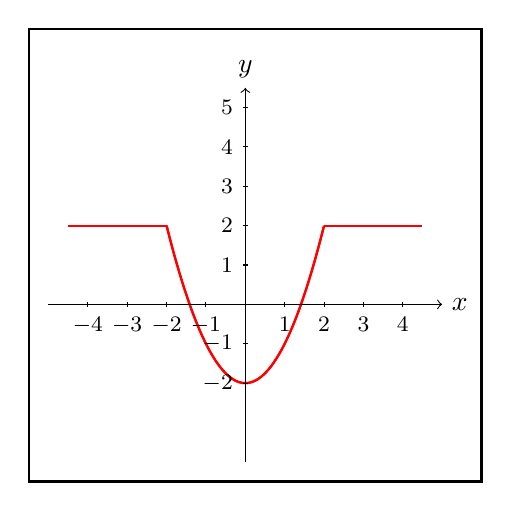
\begin{tikzpicture}[scale=0.5]
				\draw[thick] (-5.5, -4.5) rectangle (6, 7);
				% Defina o intervalo x
				\def\xmin{-3}
				\def\xmax{3}
%				
%				% Desenhe a função f(x)
%				\draw[domain=\xmin+0.4:\xmax-0.4, smooth, samples=100, blue] plot (\x, {\x*\x -2});
				
				% Desenhando a função f_2
				\draw[domain=2:4.5, thick, samples=100, red] plot (\x, {2});
				\draw[domain=-4.5:-2, thick, samples=100, red] plot (\x, {2});
				\draw[domain=-2:2, thick, samples=100, red] plot (\x, {\x*\x -2});
				\draw[domain=-2:2, thick, samples=100, red] plot (\x, {\x*\x -2});
				% Adicione rótulos aos eixos
				\draw[->] (\xmin-2,0) -- (\xmax+2,0) node[right] {$x$};
				\draw[->] (0,\xmin-1) -- (0,\xmax+2.5) node[above] {$y$};
				
                % Rótulos
				\foreach \i in {-4,-3,-2,-1,1,2,3,4}{
					\draw (\i,2pt)--(\i, -2pt) node[below]{{\footnotesize $\i$}};
				}
				
				\foreach \i in {-2, -1, 1,2,3,4,5}{
					\draw (2pt,\i)--(-2pt, \i) node[left]{{\footnotesize $\i$}};
				}
			\end{tikzpicture}
		}{
			\Fonte{Elaborado pelo autor}		}   
	\end{figure}
	
\end{env}
\end{comment}
Para que possamos entender melhor o truncamento de uma função, vamos observar o gráfico da função $g(x) = 3\cos(2x)$ apresentada na figura
\ref{fig:3cosseno_de_2x}. 
	\begin{figure}[h!]
		\centering
		\Caption{\label{fig:3cosseno_de_2x} Gráfico da função $g(x) = 3\cos (2x)$} 
		\UECEfig{}{
			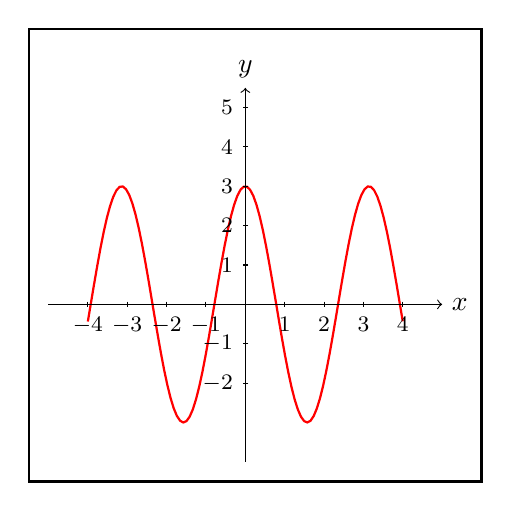
\begin{tikzpicture}[scale=0.5]
				\draw[thick] (-5.5, -4.5) rectangle (6, 7);
				% Defina o intervalo x
				\def\xmin{-3}
				\def\xmax{3}
				%				
				%				% Desenhe a função f(x)
				%				\draw[domain=\xmin+0.4:\xmax-0.4, smooth, samples=100, blue] plot (\x, {\x*\x -2});
				
				% Desenhando a função f_2
				\draw[domain=-4:4, thick, samples=100, red] plot (\x, {3*cos(2*\x r)});
				% Adicione rótulos aos eixos
				\draw[->] (\xmin-2,0) -- (\xmax+2,0) node[right] {$x$};
				\draw[->] (0,\xmin-1) -- (0,\xmax+2.5) node[above] {$y$};
				
				% Rótulos
				\foreach \i in {-4,-3,-2,-1,1,2,3,4}{
					\draw (\i,2pt)--(\i, -2pt) node[below]{{\footnotesize $\i$}};
				}
				
				\foreach \i in {-2, -1, 1,2,3,4,5}{
					\draw (2pt,\i)--(-2pt, \i) node[left]{{\footnotesize $\i$}};
				}
			\end{tikzpicture}
		}{
			\Fonte{Elaborado pelo autor}		}   
	\end{figure}
	Um truncamento faz, didaticamente falando, uma espécie de limitação no gráfico da função original.
	Ao tomarmos como constante o número real 1, vemos que o truncamento $g_1$ da função $g$, apresentada anteriormente, \enquote{amassa} o gráfico de $g$ nas ordenadas 1 e $-1$ como exposto na figura \ref{fig:truncamentog_1}.
		\begin{figure}[h!]
			\centering
			\Caption{\label{fig:truncamentog_1} Gráfico do truncamento $g_1$ } 
			\UECEfig{}{
				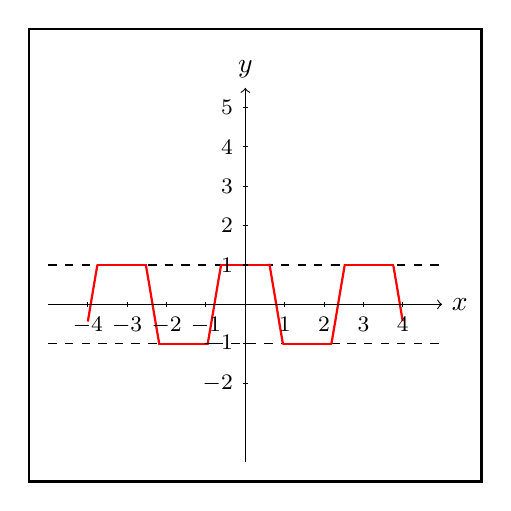
\begin{tikzpicture}[scale=0.5]
					\draw[thick] (-5.5, -4.5) rectangle (6, 7);
					% Defina o intervalo x
					\def\xmin{-3}
					\def\xmax{3}
					%				
					%				% Desenhe a função f(x)
					%				\draw[domain=\xmin+0.4:\xmax-0.4, smooth, samples=100, blue] plot (\x, {\x*\x -2});
					
					% Desenhando a função f_2
					%\draw[domain=-4:4, thick, samples=100, red] plot (\x, {3*cos(2*\x r)});
					\draw[domain=-5:5, dashed, samples=100] plot (\x, {1});
					\draw[domain=-5:5, dashed, samples=100] plot (\x, {-1});
					
					\draw[domain=-4:-3.755, thick, samples=100, red] plot (\x, {3*cos(2*\x r)});
					\draw[domain=-3.76:-2.55, thick, samples=100, red] plot (\x, {1});
					\draw[domain=-2.53:-2.18, thick, samples=100, red] plot (\x, {3*cos(2*\x r)});
					\draw[domain=-2.19:-0.96, thick, samples=100, red] plot (\x, {-1});
					\draw[domain=-0.96:-0.61, thick, samples=100, red] plot (\x, {3*cos(2*\x r)});
					\draw[domain=-0.61:0.635, thick, samples=100, red] plot (\x, {1});
					\draw[domain=0.61:0.96, thick, samples=100, red] plot (\x, {3*cos(2*\x r)});
					\draw[domain=0.96:2.19, thick, samples=100, red] plot (\x, {-1});
					\draw[domain=2.185:2.53, thick, samples=100, red] plot (\x, {3*cos(2*\x r)});
					\draw[domain=2.53:3.76, thick, samples=100, red] plot (\x, {1});]
					\draw[domain=3.76:4, thick, samples=100, red] plot (\x, {3*cos(2*\x r)});
					% Adicione rótulos aos eixos
					\draw[->] (\xmin-2,0) -- (\xmax+2,0) node[right] {$x$};
					\draw[->] (0,\xmin-1) -- (0,\xmax+2.5) node[above] {$y$};
					
					% Rótulos
					\foreach \i in {-4,-3,-2,-1,1,2,3,4}{
						\draw (\i,2pt)--(\i, -2pt) node[below]{{\footnotesize $\i$}};
					}
					
					\foreach \i in {-2, -1, 1,2,3,4,5}{
						\draw (2pt,\i)--(-2pt, \i) node[left]{{\footnotesize $\i$}};
					}
				\end{tikzpicture}
			}{
				\Fonte{Elaborado pelo autor}		}   
		\end{figure}	
	
Note que o mesmo ocorre com o truncamento $g_2$ apresentado na figura \ref{fig:truncamentog_2} onde, desta vez, $g$ é limitada pelas ordenadas $2$ e $-2$.
		\begin{figure}[h!]
			\centering
			\Caption{\label{fig:truncamentog_2} Gráfico do truncamento $g_2$ } 
			\UECEfig{}{
				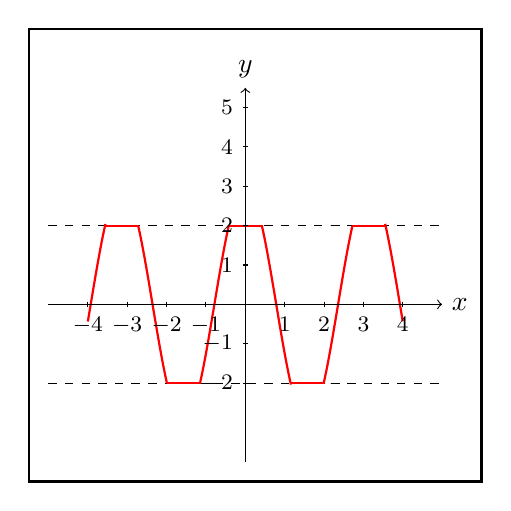
\begin{tikzpicture}[scale=0.5]
					\draw[thick] (-5.5, -4.5) rectangle (6, 7);
					% Defina o intervalo x
					\def\xmin{-3}
					\def\xmax{3}
					%				
					%				% Desenhe a função f(x)
					%				\draw[domain=\xmin+0.4:\xmax-0.4, smooth, samples=100, blue] plot (\x, {\x*\x -2});
					
					% Desenhando a função f_2
					%\draw[domain=-4:4, thick, samples=100, red] plot (\x, {3*cos(2*\x r)});
					\draw[domain=-5:5, dashed, samples=100] plot (\x, {2});
					\draw[domain=-5:5, dashed, samples=100] plot (\x, {-2});
					
					\draw[domain=-4:-3.552, thick, samples=100, red] plot (\x, {3*cos(2*\x r)});
					\draw[domain=-3.55:-2.71, thick, samples=100, red] plot (\x, {2});
					\draw[domain=-2.72:-1.99, thick, samples=100, red] plot (\x, {3*cos(2*\x r)});
					\draw[domain=-2:-1.15, thick, samples=100, red] plot (\x, {-2});
					\draw[domain=-1.15:-0.42, thick, samples=100, red] plot (\x, {3*cos(2*\x r)});
					\draw[domain=-0.43:0.43, thick, samples=100, red] plot (\x, {2});
					\draw[domain=0.42:1.16, thick, samples=100, red] plot (\x, {3*cos(2*\x r)});
					\draw[domain=1.15:2, thick, samples=100, red] plot (\x, {-2});
					\draw[domain=1.99:2.72, thick, samples=100, red] plot (\x, {3*cos(2*\x r)});
					\draw[domain=2.72:3.55, thick, samples=100, red] plot (\x, {2});]
					\draw[domain=3.552:4, thick, samples=100, red] plot (\x, {3*cos(2*\x r)});
					% Adicione rótulos aos eixos
					\draw[->] (\xmin-2,0) -- (\xmax+2,0) node[right] {$x$};
					\draw[->] (0,\xmin-1) -- (0,\xmax+2.5) node[above] {$y$};
					
					% Rótulos
					\foreach \i in {-4,-3,-2,-1,1,2,3,4}{
						\draw (\i,2pt)--(\i, -2pt) node[below]{{\footnotesize $\i$}};
					}
					
					\foreach \i in {-2, -1, 1,2,3,4,5}{
						\draw (2pt,\i)--(-2pt, \i) node[left]{{\footnotesize $\i$}};
					}
				\end{tikzpicture}
			}{
				\Fonte{Elaborado pelo autor}		}   
		\end{figure}
Assim, quanto maior o número $n$ do truncamento $g_n$ de uma função mensurável $g$, mais próximo o truncamento $g_n$ está de $g$ uma vez que a \enquote{limitação} vai desaparecendo.

Com esses resultados e observações podemos voltar a analisar o produto de duas funções com valores reais estendidos.
Considere $f,g \in \menfus$. 
Tomemos duas sequências $(f_n)$ e $(g_m)$ tais que para cada $k \in \N$, $f_k$ e $g_k$ são truncamentos de $f$ e $g$, respectivamente.
Ou seja,
	\hspace{-0.2cm}
	\begin{minipage}{0.5\linewidth}
	$$ g_p(x) =
	\left\{\begin{array}{cc}
		g(x), & \textrm{se\ } |g(x)| \leq k \\
		k, & \textrm{se\ } g(x) > k \\
		-k, & \textrm{se\ } g(x) < k 
	\end{array}\right.	
	$$	
	\end{minipage}
e
	\begin{minipage}{0.5\linewidth}
		$$ f_k(x) =
		\left\{\begin{array}{cc}
			f(x), & \textrm{se\ } |f(x)| \leq k \\
			k, & \textrm{se\ } f(x) > k \\
			-k, & \textrm{se\ } f(x) < k 
		\end{array}\right.	
		$$	
	\end{minipage}
\\

Para qualquer que seja o valor de $k \in \N$.
Pela \ref{prop:truncamento-mensurável}, $f_k$ e $g_p$ são $\cc$-mensuráveis para cada $k$ e $p$ números naturais.
Assim, pela \ref{prop:aritmetica-duas-funcoes}, $f_kg_p$ também é $\cc$-mensurável para quaisquer $k, p \in \N$.
Como mencionado anteriormente, o truncamento de uma função $f$ causa uma \enquote{limitação} em sua imagem.
Logo, se tomarmos $n$ grande o suficiente, o truncamento $f_n$ da função $f$ tende a se aproximar da própria função $f$.
Desta forma, fixemos um $m \in \N$.
Assim, para $x \in X$
$$
\lim_{k \to +\infty} \left(f_k(x)g_m(x)\right) = f(x)g_m(x) 
$$
Segue pelo \ref{cor:convergencia-de-uma-sequencia-mensuravel} que 
$fg_m \in \menfus$. 
Analogamente, para $x \in X$
$$
\lim_{m \to +\infty} \left(f(x)g_m(x)\right) 
= f(x)g(x) = (fg)(x)
$$
Concluímos, pelo mesmo corolário, que $fg \in \menfus$.
Dito isso, encerraremos esta seção apresentando a definição generalizada de mensurabilidade de uma função.

\begin{env}{Definição}
	\label{def:mensurabilidade-geral}
	Sejam $(X, \cc)$ e $(Y,\mathcal{F})$ dois espaços mensuráveis.
	Dizemos que uma função $\phi:X \to Y$ é dita mensurável se o conjunto $f^{-1}(E) = \{x \in X; f(x)\in E\} \in \cc$ para todo conjunto $E \in \mathcal{F}$ \cite{bartle}. 
\end{env}
Embora essa definição pareça ser totalmente distinta da \ref{def:mensurabilidade-funções-reais}, as duas são equivalentes no caso particular de $Y = \R$ e $\mathcal{F} = \borel$ conforme demonstrado a seguir.

\begin{env}{Proposição}
	Seja $(X, \cc)$ um espaço mensurável e $f$ uma função.
	Então $f$ é $\cc$-mensurável se, e somente se, $f^{-1}(E) \in \cc$ para todo boreliano $E$. 
\end{env}
\begin{prova}
	Suponha $f$ uma função $\cc$-mensurável. 
	Sabemos pela \ref{def:algebra-borel} que os elementos da álgebra de Borel são gerados por intervalos do tipo $(-\infty,x)$ com $x \in \R$.
	Assim, dado arbitrariamente $\alpha \in \R$ temos que
	$$
	f^{-1}(-\infty, \alpha)
	=\{x \in X; f(x) \in (-\infty, \alpha)\}
	=\{x \in X; f(x) < \alpha\}
	\footnote{Por abuso de notação, $f^{-1}(-\infty, \alpha)$ \textrm{\ indica a pré imagem de\ } $(-\infty, \alpha)$.}.
	$$
	Como $f$ é $\cc$-mensurável segue pelo \ref{teo:equiv-funcoes-mensuraveis} que $f^{-1}(-\infty, \alpha) \in \cc$.
	Note que um $E \subset \borel$ qualquer, é gerado por uniões ou intersecções de intervalos do tipo $(-\infty,x)$ com $x \in \R$ e cada pré imagem desses serão elementos  de $\cc$ por um raciocínio análogo ao que fora feito anteriormente. 
	Disso, concluímos pela \ref{prop:interseção-elementos-sigmas} e pela \ref{def:sigma-algebra} que $f^{-1}(E) \in \cc$ para todo $E \in \borel$.
	Reciprocamente se 
	$f^{-1}(-\infty, \alpha) \in \cc$ para qualquer $\alpha$ concluímos, imediatamente, que $\{x \in X; f(x) < \alpha\} \in \cc$ para todo $\alpha \in \R$.
	Portanto, $f$ é $\cc$-mensurável.
\end{prova}
%%%%%%%%%% Espaços de Medida

\section{Espaços de Medida}
Antes de definimos uma medida, lembraremos de alguns conceitos e resultados da teoria de conjuntos que nos serão úteis adiante.

\begin{env}{Definição}
\label{def:sequência-crescente-decrescente-de-conjuntos}
    Uma sequência de conjuntos $(A_n)$ é dita \textbf{não-decrescente} se $A_n \subseteq A_{n+1}$ para todo $n \in \N$.
    Caso tenhamos $A_n \supseteq A_{n+1}$ para todo $n \in \N$, dizemos que a sequência  de conjuntos é \textbf{não-crescente}
    \cite{bartle}.
\end{env}

\begin{env}{Proposição}
\label{prop:sequencia-crescente-conjuntos-resultado-A_n}
Seja $(E_n)$ uma sequência não-decrescente de conjuntos. Se $(A_n)$ é tal que $A_1 = E_1$ e $A_n = E_n - E_{n -1}$ para todo $n > 1$, então:
\begin{enumerate}[label* = (\roman*)]
    \item $A_n$ é uma sequência disjunta
        \footnote{
        	Lembre que uma sequência disjunta significa que $A_i \cap A_j = \varnothing$ para todo $i \neq j$};
    \item $E_n = \displaystyle \bigcup_{j = 1}^n A_j$;
    \item $\displaystyle \bigcup_{j = 1}^\infty E_n = \displaystyle \bigcup_{j = 1}^\infty A_n$ \cite{bartle}.
\end{enumerate}
\end{env}

\begin{prova}
    Para provar $(a)$ precisamos mostrar que para todo $n,m \in \N$ se $m \neq n$, então $A_n \cap A_m = \varnothing$.
    Suponha, sem perder generalidade, que $n > m > 1$.
    Assim, pela comutatividade e associatividade da relação de interseção e união de conjuntos segue que
    \begin{align*}
        A_m\cap A_n =& (E_m - E_{m -1}) \cap (E_n - E_{n -1})\\
        =& (E_m \cap E_{m -1}^c) \cap (E_n \cap E_{n -1}^c)\\
        =& (E_m \cap E_n) \cap ( E_{m -1}^c\cap E_{n -1}^c)\\
        =& (E_m \cap E_n) \cap \left( E_{m -1}\cup E_{n -1}\right)^c
    \end{align*}
	Como $(E_n)$ é não-decrescente, segue que $E_m \subseteq E_n$ e $E_{m-1}\subseteq E_{n-1}$.
    Deste modo, 
    $$
    (E_m \cap E_n) \cap \left( E_{m -1}\cup E_{n -1}\right)^c
    =
    E_m \cap E_{n-1}^c
    = \varnothing.
    $$
	Pois se $E_{m} \subseteq E_{n-1}$, então $E_{n-1}^c \subseteq E_{m}^c$.
	Disso, $E_{m} \subseteq E_{n-1}^c \subset E_{m} \subseteq E_{m}^c$.
    
    Provaremos agora o item $(b)$.
 	Se $m = 2$, então não há o que fazer.
 	Suponha $m > 2$.
 	Assim, 
 	\begin{align*}
 		\bigcup_{j = 1}^m A_j
 		=&
 		\bigcup_{j = 1}^m(E_j\cap E_{j-1}^c)\\
 		=&
 		E_1 \cup (E_2\cap E_{1}^c) \cup (E_3\cap E_{2}^c) \cup \cdots
 		\cup (E_m\cap E_{m-1}^c)\\
 		=&
 		\left[(E_1 \cup E_2)\cap (E_1\cup E_{1}^c)\right]
 		\cup
 		\left[(E_2 \cup E_3)\cap (E_2\cup E_{2}^c)\right]
 		\cup
 		\cdots
 		\cup 
 		\left[(E_{m-1} \cup E_m)\cap (E_{m-1}\cup E_{m-1}^c)\right]\\
 		=&
 		\left[(E_1 \cup E_2)\cap X\right]
 		\cup
 		\left[(E_2 \cup E_3)\cap X\right]
 		\cup
 		\cdots
 		\cup 
 		\left[(E_{m-1} \cup E_m)\cap X\right]\\
 		=&
 		(E_1 \cup E_2)
 		\cup
 		(E_2 \cup E_3)
 		\cup
 		\cdots
 		\cup 
 		(E_{m-1} \cup E_m)\\
 		=&
 		E_1 \cup E_2 \cup E_3\cup 
 		\cdots
 		\cup E_{m-1} \cup E_m\\
 		=& E_m.
 	\end{align*}
	A última igualdade ocorre pelo fato de $(E_n)$ ser não-decrescente.
	Assim, $E_1 \subseteq E_2 \subseteq \cdots \subseteq E_m$.
	
    Por fim, $(c)$ é um resultado imediato, pois $ x \in \displaystyle \bigcup_{j = 1}^\infty E_j$ se, e somente se, 
    existe um $n_0 \in \N$ tal que $x \in E_{n_0}$. 
    Pelo item $(b)$, isso só ocorre se $x \in \displaystyle \bigcup_{j = 1}^{n_0}A_j$.
    Mas isso é equivalente à dizer que existe um $k$ com $1\leq k\leq n_0$ tal que $x \in A_k$.
    Como $k \in \N$ isso acontece se, e somente se, $x \in A_k$ para algum $k \in \N$.
    Portanto $x \in \displaystyle \bigcup_{j = 1}^\infty A_j$.
\end{prova}

\begin{env}{Proposição}
\label{prop:sequencia-decrescente-conjuntos-resultado-A_n}
Seja $(F_n)$ uma sequência não-crescente de conjuntos. 
Se $(E_n)$ é tal que $E_n = F_1 - F_n$ para todo $n \in \N$, então $(E_n)$ é não-decrescente e 
$\displaystyle \bigcup_{j = 1}^\infty E_n = \displaystyle F_1 - \bigcap_{j = 1}^\infty F_n$
\cite{bartle}.
\end{env}

\begin{prova}
    Queremos mostrar que $(E_n)$ é não-decrescente, isto é, $E_n \subseteq E_{n+1}$ para todo $n \in \N$.
    Dado um $n \in \N$, tome $x \in E_n$. 
    Logo, $x \in F_1$ e $x \notin F_n$, por construção.
    Como $(F_n)$ é não-crescente, ocorre $F_{n} \supseteq F_{n+1}$. 
    Assim, $x \notin F_n \Rightarrow x \notin F_{n+1}$.
    Com isso, $x \in F_1$ e $x \notin F_{n+1}$, ou seja,
    $x \in E_{n+1}$.
    Desta maneira, $E_n \subseteq E_{n+1}$ para qualquer $n \in \N$, como queríamos.
    Além disso, perceba que
$$
    	\bigcup_{j = 1}^\infty E_n 
    	= 
    	\bigcup_{j = 1}^\infty (F_1-F_n)\\
    	= 
    	\bigcup_{j = 1}^\infty (F_1 \cap F_n^c)\\
    	= 
    	F_1 \cap \left(\bigcup_{j = 1}^\infty F_n^c\right)\\
    	= 
    	F_1 \cap \left(\bigcap_{j = 1}^\infty F_n\right)^c\\
    	= 
    	F_1 -\bigcup_{j = 1}^\infty F_n
$$
\end{prova}

\begin{env}{Proposição}
	\label{prop: duas partições}
	Se $\displaystyle \bigcup_{j = 1}^n E_j$ e $\displaystyle \bigcup_{k = 1}^m F_k$ são duas partições distintas de um conjunto $X$, então
	para cada $j \in I_n$ tem-se $E_j = \displaystyle \bigcup_{k = 1}^m (E_j \cap F_k)$
	\cite{bartle}.
\end{env}
\begin{prova}
	Fixemos um $j_0 \in I_n$.
	Assim, temos que $\displaystyle x \in \bigcup_{k = 1}^m (E_{j_0} \cap F_k)$ implica que existe um $k_0 \in I_m$ tal que  $x \in E_{j_0}\cap F_{k_0}$.
	Logo, $x \in E_{j_0}$ e $x \in F_{k_0}$, isto é, $x \in E_{j_0}$.
	Reciprocamente, se $y \in X$, então para algum $j_1 \in I_n$, $y \in E_{j_1}$, pois $\{E_j\}$ formam uma partição de $X$.
	Como $\{F_k\}$ também é uma partição de $X$, deve existir um $k_1 \in I_m$ tal que $x \in F_{k_1}$.
	Assim, $x \in E_{j_1} \cap F_{k_1}$. 
	Desta forma, existe um $k_1 \in I_m$ tal que $x \in \displaystyle \bigcup_{k = 1}^m (E_{j_1} \cap F_{k})$ como queríamos.	 
\end{prova}

\begin{env}{Definição}
\label{def:medida}
    Uma medida é uma função $\mu: (X, \mathcal{C}) \to \xreta$ tal que satisfaz as seguintes condições:
    \begin{enumerate}[label* = (\roman*)]
        \item $\mu(\varnothing) = 0$;
        \item $\mu(A) \geq 0, \ \forall \ A \in \mathcal{C}$;
        \item Se $(A_n)$ é uma sequência disjunta de elementos de  $\mathcal{C}$, então 
        $\displaystyle\mu\left(\bigcup_{n = 1}^\infty A_n\right) = \sum_{n = 1}^\infty\mu(A_n)$ \cite[p.19, tradução nossa]{bartle}.
        
    \end{enumerate}
\end{env}

O valor de $\mu$ pode ser igual à $+\infty$ para algum conjunto $A \in \mathcal{C}$.
Quando temos que $\mu(E) < +\infty$ para qualquer que seja o conjunto $E \in \mathcal{C}$, dizemos que temos uma medida finita.

\begin{env}{Definição}
	\label{def:espaço-de-medida}
	Dizemos que uma tripla ordenada $(X, \mathcal{C}, \mu)$ constituída por um conjunto $X$, uma \sigal $\mathcal{C}$ desse conjunto e uma medida $\mu$ sobre o espaço mensurável $(X, \mathcal{C})$ é um espaço de medida \cite{bartle}.
\end{env}


% Exemplos de medida

\begin{env}{Exemplo}
    Sejam $X$ um conjunto e $\mathcal{C}$ a \sigal formada por todos os subconjunto de $X$.    
    Defina $\mu_1, \mu_2:\mathcal{C} \to \xreta$ pondo $\mu_1(A) = 0$ para qualquer  $A \in \mathcal{C}$ e 
    $\mu_2$ é  pondo 
	$$\mu_2(A) = \left\{\begin{array}{cc}
	0, & \textrm{\ se \ } A = \varnothing \\
	+\infty,& \textrm{\ se \ } A \neq \varnothing
	\end{array}\right.$$
	Sendo definidas dessa forma, as funções $\mu_1$ e $\mu_2$ são medidas.
	\end{env}

De fato, em ambas as condições \textit{(i)} e \textit{(ii)} são trivialmente satisfeitas.
Para a condição \textit{(iii)}, temos que qualquer sequência disjunta $(A_n)$ acarretará que

$$\mu_1\left(\bigcup_{n = 1}^\infty A_n\right) = 0 = \sum_{n = 1}^\infty \mu_1(A_n) $$
Para $\mu_2$ temos dois casos possíveis.
Se  $\displaystyle \bigcup_{n = 1}^\infty A_n  = \varnothing$, então $\mu_2\left(\displaystyle \bigcup_{n = 1}^\infty A_n\right) = 0$. Entretanto isso ocorre somente se $A_j = \varnothing$ para todo $j \in \N$.
Logo, 

$$\sum_{n = 1}^\infty \mu_2(A_n) = \sum_{n = 1}^\infty \mu_2(\varnothing) = 0$$

Caso $\displaystyle \bigcup_{n = 1}^\infty A_n  \neq  \varnothing$, dentre os termos da sequência $(A_n)$, deve existir pelo menos um $p \in \N$ tal que $(A_p) \neq \varnothing$.
Assim, $\mu(A_j) = +\infty$ para algum $p \in \N$ acarretando que  $\mu_2\left(\displaystyle \bigcup_{n = 1}^\infty A_n\right) =~+\infty$.

Ademais, na soma $\displaystyle \sum_{n = 1}^\infty \mu_2(A_n)$ só teremos soma dos termos $0 + (+ \infty)$ ou $(+\infty) + (+\infty)$.
Desta forma, $\displaystyle \sum_{n = 1}^\infty \mu_2(A_n) = +\infty$.
Portanto $\mu_1$ e $\mu_2$ são medidas.

% Probabilidade
\begin{env}{Exemplo}
	Seja $(\Omega, \cc)$ um espaço mensurável.
	A função $\mathcal{P}:\cc \to [0,1]$ é dita uma probabilidade se satisfaz as propriedades:
	\begin{enumerate}[label* =(\textit{K\arabic*})]
		\item $\mathcal{P}(\Omega) = 1$;
		\item $\mathcal{P}(A) \geq 0,\ \forall\  A \in \cc$;
		\item Se $(A_n)$ é uma sequência disjunta de elementos de  $\mathcal{C}$, então 
		$\displaystyle\mathcal{P}\left(\bigcup_{n = 1}^\infty A_n\right) = \sum_{n = 1}^\infty\mathcal{P}(A_n)$
		\cite[p.11, adaptação nossa]{magalhaes}
		\footnote{As propriedades \textit{K1, K2} e \textit{K3} são chamadas de \textit{Axiomas de Kolmogorov}}.
	\end{enumerate}
\end{env}

Observe que as condições da \textit{(ii)} e \textit{(iii)} da \ref{def:medida} são satisfeitas, por definição, na função de probabilidade.
Resta provar que $\mathcal{P}(\varnothing) = 0$.
Assim, com o auxilio das propriedades \textit{(K1)} e \textit{(K3)}, segue que 
$$
\pp(\Omega)
= 
\pp(\Omega \cup \varnothing)
= 
\pp(\Omega) + \pp(\varnothing)
\Rightarrow
\pp(\Omega)
= 
\pp(\Omega) + \pp(\varnothing)
\Rightarrow
\pp(\varnothing) = 0.
$$
Portanto a função probabilidade é uma medida.
Neste caso, o espaço de medida $(\Omega, \cc, \pp)$ é chamado de espaço de probabilidades.
Além disso, uma função $\cc$-mensurável pela \ref{def:mensurabilidade-geral} em um espaço de probabilidades é chamada de variável aleatória.

% Unidade de Medida Concentrada em p
\begin{env}{Exemplo}\textbf{(Unidade de Medida Concentrada em $p$)}
\label{ex:medida-concentrada-em-p}
    Seja $(X, \mathcal{C})$ um espaço mensurável onde $\cc = \mathcal{P}(X)$ e $p$ um elemento de $X$.
    Defina $\mu: \mathcal{C} \to \xreta$  como sendo

$$\mu(A) = \left\{\begin{array}{cc}
0, & \textrm{\ se \ } p \notin A \\
1, & \textrm{\ se \ } p \in A 
\end{array}\right.$$


Então $\mu$ é uma medida.
Verdadeiramente, observe que $p \notin \varnothing$, ou seja, $\mu(\varnothing) = 0$.
Trivialmente, tem-se $\mu(A) \geq 0,\ \forall A \in \mathcal{C}$, pela construção de $\mu$.


\end{env}
\begin{comment}
	

% A função característica é uma medida
\begin{env}{Exemplo}
	\label{ex: função característica é uma medida}
	Seja $\cc$ uma \sigal e $E \subset \cc$.
	A função característica $\chi_{E}: \cc \to \R$ é uma medida sobre $\cc$.
	De fato, $\chi_{\varnothing} = 0$, pois não há elementos em $\varnothing$.
	Pela definição de função característica, temos que $\chi_E(x) \neq 0$ para qualquer que seja $E \in \cc$.
	Por fim, Se $(E_n)$ é uma sequência disjunta de elementos de $\cc$, sempre temos $\chi_{\bigcap_{n \in \N}E_n} = 0$.
	Caso $\chi_{\bigcup_{n \in \N}E_n}(x) = 0$, então $x \notin \bigcup_{n \in \N}E_n$. 
	Logo, $x \notin E_n,\ \forall n \in \N$.
	Logo, $\chi_{E_n}(x) = 0$ para qualquer que seja $n \in \N$, 
	Com isso, $\dsum_{n \in \N} \chi_{E_n}(x) = 0 = \chi_{\bigcup_{n \in \N}E_n}(x)$.
	
	Caso ocorra que  $\chi_{\bigcup_{n \in \N}E_n}(x) = 1$, então existe um $n_0 \in \N$ tal que $ x \in E_{n_0}$.
	Como a sequência de conjuntos é disjunta, o $n_0$ é único.
	Logo, $x \notin E_p$ para qualquer $p \neq n_0$, ou seja, $\chi_{E_p}(x) = 0, \ \forall p \neq n_0$.
	Com isso, $\dsum_{p \neq n_0} \chi_{E_p}(x) + \chi_{E_{n_0}}(x) = 0 + 1 =  \chi_{\bigcup_{n \in \N}E_n}(x)$.
	Em todo caso, $\chi_{\bigcup_{n \in \N}E_n}(x) = \dsum_{n \in \N} \chi_{E_n}(x)$. 
	Portanto, $\chi_E$ é uma medida.
\end{env}
\end{comment}

% Medida de contagem

\begin{comment}
	\begin{env}{Exemplo}
		Seja $X = \N$ e $\mathcal{C}$ sendo o conjunto das partes de $\N$. 
		para $A \in \mathcal{C}$, definimos $\mu(A)$ por meio da sua cardinalidade, isto é, se $A$ é finito, então $\mu(A)$ é quantidade de elementos de $A$. Caso contrário, $\mu(A) = +\infty$.	
	\end{env}
\end{comment}


\begin{env}{Proposição}
	\label{prop: medida com partição}
	Se $\displaystyle \bigcup_{j \in I_n} E_j$ e $\displaystyle\bigcup_{k \in I_m} F_k$ são duas partições de um conjunto $X$, então 
	$\displaystyle \mu(E_j) 
	= 
	\sum_{k = 1}^{m} \mu(E_j\cap F_k)$.
\end{env}

\begin{prova}
	Dado $j \in I_n$, pela \ref{prop: duas partições}, temos que
	$E_j = \displaystyle \bigcup_{k = 1}^m (E_j\cap F_k)$.
	Como $\{F_k\}$ é uma partição, para $k,l \in I_m$, temos
	$(E_j\cap F_p) \cap (E_j\cap F_l) = \varnothing$ para todo $l$ e $p$ com  $l \neq p$.
	Ou seja, a sequência formada por $(E_j\cap F_k)$ com $k \in I_m$ é disjunta.
	Como $\mu$ é uma medida, segue que
	$$
	\mu(E_j)
	=
	\mu\left(\bigcup_{k = 1} (E_j\cap F_k)\right)
	=
	\sum_{k = 1}^{m}\mu(E_j\cap F_k)
	$$
\end{prova}

\begin{comment}
	

\begin{env}{Proposição}
	\label{prop: igualdade da caracteristica como medida}
	Se $\displaystyle \bigcup_{j \in I_n} E_j$ e $\displaystyle\bigcup_{k \in I_m} F_k$ são duas partições de um conjunto $X$, então 
	$\displaystyle \chi_{E_j} = \sum_{k = 1}^{m} \chi_{(E_j\cap F_k)}$.
\end{env}

\begin{prova}
	Pela \ref{prop: igualdade da caracteristica como medida}, $\chi$ é uma medida. Segue pela \ref{prop: medida com partição} que
	$\displaystyle \chi_{E_j} = \sum_{k = 1}^{m} \chi_{(E_j\cap F_k)}$.
\end{prova}
\end{comment}

% Teorema
\begin{env}{Teorema}
\label{teo:medida-diferença}
	Seja $\mu$ uma medida definida sobre uma \sigal $\mathcal{C}$.
	Se $A$ e $B$ são elementos de $\mathcal{C}$ e $A \subset B$, então $\mu(A) \leq \mu(B)$.
	Se $\mu(A) < +\infty$, então $\mu(B-A) = \mu(B) - \mu(A)$ \cite{bartle}.
\end{env}

\begin{prova}
	Suponha que $A \subset B$, então $B = A \cup (B - A)$ e $A \cap (B - A) = \varnothing$. Segue pela propriedade $(ii)$ da \ref{def:medida} que 
	$$\mu(B) = \mu(A) + \mu(B-A)$$
	Lembre que $B-A = B\cap A^c$ e $A \in \mathcal{C} \Rightarrow A^c \in \mathcal{C}$.
	Além disso, como $B \in \mathcal{C}$ temos que $ B\cap A^c = B - A \in \mathcal{C}$.
	Com isso, $\mu(B-A) \geq 0$.
	Segue que $\mu(B) \geq \mu(A)$.
	Observe que se $\mu(A) < \infty$, temos que 

	$$\mu(B) = \mu(A) + \mu(B-A) 
 \Leftrightarrow \mu(B) - \mu(A) =  \mu(B-A)
 $$
Como desejávamos.
\end{prova}

\begin{env}{Proposição}
\label{prop:limite-sequencia-crescente}
Seja $\mu$ uma medida definida sobre uma \sigal $\mathcal{C}$.
Se $(E_n)$ é uma sequência não-decrescente de $\mathcal{C}$, então $\mu\left(\displaystyle \bigcup_{n = 1}^\infty E_n\right) = \dlim_{n \to \infty} \mu(E_n)$
\cite{bartle}.
\end{env} 

\begin{prova}
    Ora, se $\mu(E_n) = +\infty$, para algum $n \in \N$, ambos os lados da equação acima são $+\infty$.
    Desta forma, vamos supor que $\mu(E_n) < +\infty$ para todo $n \in \N$.
    Com isso, vamos construir uma sequência $(A_n)$ pondo $A_1 = E_1$ e $A_n = E_n - E_{n-1}$ para qualquer $n>1$.
    Então pela \ref{prop:sequencia-crescente-conjuntos-resultado-A_n}, $(A_n)$ é uma sequência disjunta, temos 
    $\displaystyle E_n = \bigcup_{j = 1}^n A_j$ e 
    $\displaystyle\bigcup_{j = 1}^\infty E_j = \bigcup_{j = 1}^\infty A_j$.
    Como $\mu$ contavelmente aditiva, 
    $$\mu\left(\bigcup_{n = 1}^\infty E_n\right)
    =\mu\left(\bigcup_{n = 1}^\infty A_n\right)
    = \sum_{n = 1}^\infty \mu(A_n)
    = \lim_{m \to +\infty}\sum_{n = 1}^m \mu(A_n)$$
    Pelo  \ref{teo:medida-diferença} vemos que $\mu(A_n) = \mu(E_n) - \mu(E_{n - 1 })$, para $n > 1$.
    Assim, 
    
    \begin{align*}
        \lim_{m \to +\infty}\sum_{n = 1}^m \mu(A_n)
        =&
        \lim_{m \to +\infty}(\mu(A_1) + \mu(A_2) + \cdots +\mu(A_m))\\
        =&
        \lim_{m \to +\infty}(\mu(E_1) + \mu(E_2 - E_1) + \cdots +\mu(E_m - E_{m-1}))\\
        =&
        \lim_{m \to +\infty}(\mu(E_1) + \mu(E_2) - \mu(E_1) + \cdots +\mu(E_m) - \mu(E_{m-1}))\\
        =&
        \lim_{m \to +\infty}(\mu(E_1) - \mu(E_1) + \mu(E_2)  + \cdots  - \mu(E_{m-1}) +\mu(E_m) )\\
        =&
        \lim_{m \to +\infty} \mu(E_m)
    \end{align*}
    Segue que $\mu\left(\displaystyle \bigcup_{n = 1}^\infty E_n\right) = \dlim_{n \to \infty} \mu(E_n)$.




% Note que $H_2 = A_2 - A_1$ e $H_3 = A_3 - A_2$. Logo, $H_1 \cup H_2 \cup H_3$
% Assim, 

% % \begin{align*}
%     \bigcup_{n = 1}^4 H_n =&
%     \bigcup_{n = 1}^4 (A_n - A_{n-1})\\
%     =&
%     \bigcup_{n = 1}^4 \left(A_n \cap (A_{n-1})^c\right)\\
%     =&
%     \left(A_1 \cap (A_{1-1})^c\right)\\
    
% \end{align*}


\end{prova}

\begin{env}{Proposição}
Seja $\mu$ uma medida definida sobre uma \sigal $\mathcal{C}$.
Se $(B_n)$ é uma sequência não-crescente de $\mathcal{C}$ e $\mu(B_1) < +\infty$, então 
$\mu\left(\displaystyle \bigcap_{n = 1}^\infty B_n\right) = \dlim_{n \to \infty} \mu(B_n)$ \cite{bartle}.
\end{env} 
\begin{prova}
    Defina uma sequência $(T_n)$ de elementos de $\mathcal{C}$ pondo $T_n = B_1 - B_n$ para qualquer que seja $n \in \N$.
    Pela \ref{prop:sequencia-decrescente-conjuntos-resultado-A_n}, $(T_n)$ é não-decrescente.
    Assim, aplicando o a \ref{prop:limite-sequencia-crescente} temos que 
    $$
    \mu\left(\bigcup_{n \in \N} T_n\right) = \lim_{n \to +\infty} \mu(T_n)
    $$
    Usando o \ref{teo:medida-diferença}, obtemos
    $$
    \lim_{n \to +\infty} \mu(T_n) = \lim_{n \to +\infty} [\mu(B_1) - \mu(B_n)] = \mu(B_1) - \lim_{n \to +\infty} \mu(B_n)
    $$
    Segue pela \ref{prop:sequencia-decrescente-conjuntos-resultado-A_n} que 
    $$
    \lim_{n \to +\infty} \mu(T_n) = \mu(B_1) - \mu\left(\bigcap_{n \in \N} B_n\right)
    $$
    Combinando as duas equações obtemos que
    \begin{align*}
        \mu(B_1) - \lim_{n \to +\infty} \mu(B_n) = \mu(B_1) - \mu\left(\bigcap_{n \in \N} B_n\right)
    \end{align*}
    Portanto, $\displaystyle \lim_{n \to +\infty} \mu(B_n) = \mu\left(\bigcap_{n \in \N} B_n\right)$
\end{prova}

Vimos quando tratamos de \sigals a \sigal de Borel que é muito relevante para o estudo da reta real.
Da mesma forma, existe uma medida que é indispensável para o mesmo contexto.
Essa, por sua vez, não será demonstrada a titulo de simplificação do trabalho, mas será enunciada aditante pela importância. 
\begin{env}{Teorema}
	\label{teo: medida de lebesgue}
	Sendo $(\R, \borel)$ um espaço mensurável, existe uma única medida $\lambda$ definida sobre $\borel$ que coincide com o comprimento dos intervalos abertos \cite[p.20, tradução nossa, adaptação nossa]{bartle}
	\footnote{No original: If $X = \textbf{R}$ and $\textbf{X} = \textbf{B}$, the Borel algebra, then [...] there exists a unique measure $\lambda$ defined on $\textbf{B}$ which coincides with length on open intervals.}.
\end{env}

Em termos práticos, se $E$ é um intervalo real não vazio $(a,b)$, então $\lambda(E) = b - a$.
Esta medida recebe o nome de Medida de Lebesgue. 
Embora tenha tido a necessidade de utilizar o sistema da reta estendida para definirmos uma medida, existem conjuntos tão pequenos que sua medida é desprezível.
À esses damos o nome de conjunto de medida nula.
Formalmente,

\begin{env}{Definição}
	\label{def:conjunto-medida-nula}
	Seja $(X, \cc, \mu)$ um espaço de medida.
	Dizemos que um conjunto $E \in \cc$ tem medida nula em relação à medida $\mu$ se $\mu(E) = 0$.
\end{env}

Podemos usar este conceito de \enquote{quase todo ponto} ou \enquote{quase todo lugar} para qualquer proposição que queiramos desde que ela não seja válida apenas em um subconjunto de medida nula \cite{bartle}.
\begin{env}{Proposição}
	\label{prop:medida-nula-subconjunto}
	Seja $(X, \cc, \mu)$ um espaço de medida.
	Se $\mu(X) = 0$ e $Y \subset X$, então $\mu(Y) = 0$ \cite[p.343, adaptação nossa]{elon}.
\end{env}
\begin{prova}
	Note que $(Y \cap X) \subset X$, pois $ Y \cap X = Y$.
	Assim, pelo \ref{teo:medida-diferença}, temos que
	$
	\mu(Y) = \mu(X \cap Y) \leq \mu(X) = 0
	$.
	Logo, $\mu(Y) \leq 0$.
	Segue que $\mu(Y) = 0$, pois a medida é uma função não negativa.
	\vspace{-0.4cm}
\end{prova}

\begin{env}{Proposição}
	\label{prop:medida-nula-união}
	Seja $(X, \cc, \mu)$ um espaço de medida e $\{E_n\}$ uma sequência disjunta de elementos de $\cc$.
	Se $Y = \displaystyle\bigcup_{n \in \N}E_n$ e $\mu(E_n) = 0$ para todo $n \in \N$, então $\mu(Y) = 0$ \cite[p.343, adaptação nossa]{elon}.
\end{env}
\begin{prova}
	Analogamente à proposição anterior segue, imediatamente, que
	$$
	\mu(Y)
	=
	\mu\left(\bigcup_{n \in \N}E_n\right)
	=
	\sum_{n = 1}^\infty \mu(E_n)
	= 0.
	$$
	Assim,
	$\mu(Y)\leq 0$. Portanto, $\mu(Y) = 0$.
\end{prova}

Como exemplo, temos por definição, que $\varnothing$ tem medida nula, pois para qualquer medida $\mu$, $\mu(\varnothing) = 0$.
Mostraremos a seguir um exemplo menos trivial:

\begin{env}{Exemplo}
	Se $X \subset \R$ é um conjunto discreto, então tem medida nula com respeito à medida $\lambda$ de Lebesgue.
	De fato, se $X$ é discreto, então é formado por pontos isolados.
	Assim, se $a \in X$, então pode ser representado degeneradamente, por 
	$\{a\} = [a,a]$.
	Logo, $\lambda(\{a\}) = a - a = 0$.
	Assim, o conjunto $X$ é dado pela reunião enumerável de seus pontos e todos têm medida nula. 
	Segue pela \ref{prop:medida-nula-união} que $X$ tem medida nula.
\end{env}


 
% Espaços de Medida

%Uma vez que já foram bem explorados os espaços mensuráveis bem como os espaços de medida, nosso objetivo neste capítulo é medir 
